\section{Introduction}

Complementation is a very fundamental graph operation and 
modifying a graph by complementing an induced subgraph to satisfy certain properties is a natural algorithmic problem on graphs. The operation of complementing an induced subgraph, known as subgraph complementation, is introduced by Kami{\'n}ski et al.~\cite{DBLP:journals/dam/KaminskiLM09} in connection with clique-width of graphs. For a class $\mathcal{G}$ of graphs, the objective of \textsc{Subgraph Complementation to} $\mathcal{G}$ is 
to find whether there exists a subset $S$ of the vertices of the input graph $G$ such that complementing the subgraph induced by $S$ in $G$ results in a graph in $\mathcal{G}$.  Fomin et al.~\cite{DBLP:journals/algorithmica/FominGST20} studied this problem on various classes $\mathcal{G}$ of graphs.
They obtained that the problem can be solved in 
polynomial-time when $\mathcal{G}$ is bipartite, d-degenerate, or co-graphs. In addition to this, they 
proved that the problem is NP-complete when $\mathcal{G}$ is the class of all regular graphs.
Antony et al.~\cite{DBLP:journals/algorithmica/AntonyGPSSS22} studied this problem when $\mathcal{G}$ is the class of $H$-free graphs (graphs without any induced copies of $H$). They proved that the problem
is polynomial-time solvable when $H$ is a complete graph on $t$ vertices. They also proved that the problem is NP-complete when $H$ is a star graph on at least 6 vertices or a path or a cycle on at least 7 vertices. Later Antony et al.~\cite{DBLP:conf/latin/AntonyPSS22} proved that
the problem is polynomial-time solvable when $H$ is paw, and NP-complete when $H$ is a tree, except for 41 trees of at most 13 vertices. It has been proved~\cite{DBLP:journals/algorithmica/AntonyGPSSS22,DBLP:conf/latin/AntonyPSS22}
that none of these hard problems admit subexponential-time algorithms (algorithms running in time $2^{o(n)}$), assuming the Exponential Time Hypothesis. 


Fomin et al.~\cite{DBLP:journals/algorithmica/FominGST20} 
proved that the problem is polynomial-time solvable not only when $\mathcal{G}$ is the class of $d$-degenerate graphs but also when $\mathcal{G}$ is any subclass of $d$-degenerate graphs recognizable in polynomial-time. 
This implies that the problem is polynomial-time solvable when $\mathcal{G}$ is the class of $r$-regular
graphs or the class of graphs with maximum degree at most $r$ (for any constant $r$). They asked whether the problem can be solved in polynomial-time when $\mathcal{G}$ is the class of graphs with minimum
degree at least $r$, for a constant $r$. We resolve this positively and obtain a stronger result - a simple quadratic kernel for the following parameterized problem: Given a graph $G$ and an
integer $k$, find whether $G$ can be transformed into
a graph with minimum degree at least $k$ by subgraph
complementation (here the parameter is $k$).  
The result follows from an observation that if $G$ has 
more than $2k^2-2$ vertices, then it is a yes-instance of the problem.

When $\mathcal{G}$ is the class of graphs without any 
induced copies of the star graph on $t+1$ vertices (for any fixed $t\geq 3$) and the diamond (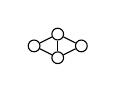
\begin{tikzpicture}[myv/.style={circle, draw, inner sep=1.5pt}]
    \node (o) at (0,0) {};
    \node[myv] (v1) at (0,0.15) {};
    \node[myv] (v2) at (0,-0.15) {};
    \node[myv] (v3) at (-0.3,0) {};
    \node[myv] (v4) at (0.3,0) {};

    \draw (v1) -- (v2);
    \draw (v1) -- (v3);
    \draw (v1) -- (v4);
    \draw (v2) -- (v3);
    \draw (v2) -- (v4);

\end{tikzpicture}), we obtain a polynomial-time algorithm. 
When $t=3$ this graph class is known as linear domino and is the class of line graphs of triangle-free graphs. Cygan et al.~\cite{DBLP:journals/mst/CyganPPLW17} have studied the polynomial kernelization of edge deletion problem for this target graph class. When $t=4$, the graph class is the line graphs of linear hypergraphs of rank 3. 
The technique that we use is similar to that given in \cite{DBLP:journals/algorithmica/AntonyGPSSS22} and \cite{DBLP:conf/latin/AntonyPSS22} for obtaining 
polynomial-time algorithms when $\mathcal{G}$ is $H$-free, for $H$ being a complete graph on $t$ vertices or a paw. Our result is in contrast with the result
by Antony et al.~\cite{DBLP:journals/algorithmica/AntonyGPSSS22} that the problem is NP-complete and cannot be solved in subexponential-time (assuming the Exponential Time Hypothesis) when $H$ is a star graph on $t+1$ vertices, for every constant $t\geq 5$. 

